
\documentclass{beamer}
\usepackage[latin1]{inputenc}
%\usetheme{Montpellier}
%\usetheme{Boadilla}
%\usecolortheme[RGB={204,51,255}]{structure}
%\usecolortheme[named=purple]{structure}
\usecolortheme[RGB={62,128,62}]{structure}
%\definecolor{dark}{rgb}{0.3,0.15,0.3}
%\definecolor{light}{rgb}{0.8,0.6,0.8}
%\definecolor{reddish}{rgb}{.5,0.15,0.15}
\definecolor{dark}{rgb}{0.5,0.3,0.4}
%\definecolor{light}{rgb}{0.8,0.6,0.8}
\definecolor{reddish}{rgb}{.7,0.25,0.25}
\definecolor{greenish}{rgb}{.25,0.7,0.25}
\definecolor{blueish}{rgb}{.25,0.25,0.7}
\definecolor{purple}{rgb}{.5,0.0,0.5}
\usepackage{graphicx}
\usepackage{pstricks}

\setbeamertemplate{navigation symbols}{}

\newcommand{\crish}{\color{reddish}}
\newcommand{\cbla}{\color{black}}
\newcommand{\cred}{\color{red}}
\newcommand{\cblu}{\color{blue}}

\usepackage{tikz}
\usetikzlibrary{arrows,decorations.markings,positioning}
\usepackage{epstopdf}

\title[Computational Neuroscience 2]{Computational Neuroscience 2}
\author{PHPH20007}
\institute{\texttt{github.com/conorhoughton/PHPH20007}}
\date{May 2019}

\begin{document}

\maketitle

\begin{frame}{Modelling}
This is an example of a model that explains what might be happening without giving a detailed simulation of the individual components involved.
  \end{frame}

\begin{frame}{Modelling}
  Here we look at the hippocampus and introduce a more top down style
  of modelling.
\end{frame}
  
\begin{frame}{The hippocampus}
  \begin{center}
    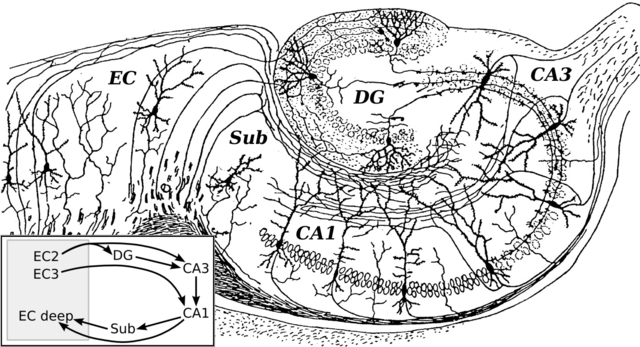
\includegraphics[height=8cm]{hippocampus.png}
  \end{center}
      \vfill
  \flushright{\tiny{image from wikipedia, originally due to Cajal}}
\end{frame}

\begin{frame}{The role of the hippocampus}
  \begin{center}
    
\includegraphics[height=8cm]{finding_lost_items.jpg}
  \end{center}
      \vfill
  \flushright{\tiny{www.wikihow.life/Find-Things-You-Lost}}
\end{frame}


\begin{frame}{The role of the hippocampus}
  \begin{center}
    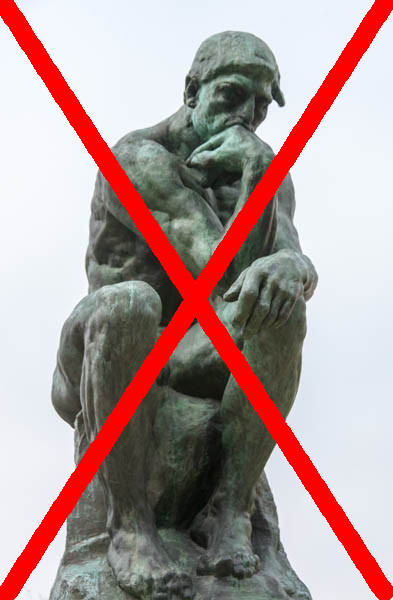
\includegraphics[height=8cm]{the_thinker_cancelled.png}
  \end{center}
      \vfill
  \flushright{\tiny{image of Rodin's \textsl{The Thinker} from wikipedia}}
\end{frame}

\begin{frame}{Parts of the hippocampus}
\begin{itemize}
\item \textbf{Cornu Ammonis (CA)} - meaning the \textsl{horn of Ammon}. The CA is usually divided
  into four regions, labelled CA1 through to CA4.
\item \textbf{Dentate Gyrus (DG)}- gyrus is the name given to the ridges in the
  cortex, dentate means \textsl{with teeth}.
\end{itemize}
In addition, the main input to the hippocampus comes from the
\begin{itemize}
\item \textbf{Entorhinal Cortex (EC)} - entorhinal means \textsl{near the smell processing area}. 
\end{itemize}
and in this discussion this will be treated along with the hippocampus
since it partiticipates in hippocampal processing.
\end{frame}

\begin{frame}{How the hippocampus is connected}
  \begin{center}
\begin{tikzpicture}[->,>=stealth']

 \node[state,text width=3cm](DG) 
 {\textbf{DG}
  };
  
 \node[state, 
 node distance=6cm,
 text width=3cm,  
 right of=DG,     
 yshift=+3cm](CA3)
 {\textbf{CA3}
 };
 
 \node[state,
  below of=CA3,
  yshift=-2cm,
  anchor=center,
  text width=3cm] (EC) 
 {\textbf{EC}
 };

 \node[state,
  right of=CA3,
  node distance=5cm,
  anchor=center,
text width=3cm] (CA1) 
 {\textbf{CA1}
 };

 \path (DG) 	edge[bend left=20]  (CA3)
       (EC)  edge (DG)
 (EC)  edge (CA3)
 (EC)  edge[bend left=20] (CA1)
 (CA1)  edge[bend left=20] (EC)
 (CA3)  edge (CA1)
 (CA3)  	edge[loop above]   (CA3)
;

\end{tikzpicture}
\end{center}
\end{frame}

\begin{frame}{Cells}
  The dentate gyrus is composed of granule cells, CA3 of pyramidal cells. DG is thought of a \textsl{feed-forward} whereas CA3 is highly \textsl{recurrent}.
  \begin{center}
    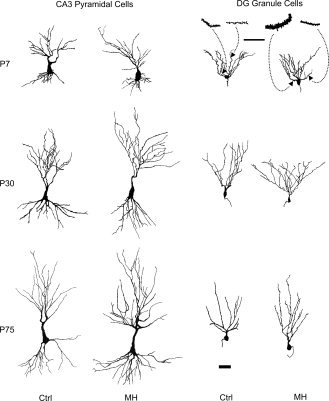
\includegraphics[height=6cm]{cells.jpg}
  \end{center}
      \vfill
  \flushright{\tiny{from 10.1002/jnr.21580}}
\end{frame}




\end{document}

